\documentclass[12pt]{article}

\usepackage{sbc-template}
\usepackage[T1]{fontenc}
\usepackage[utf8]{inputenc}
\usepackage[brazil]{babel}
\usepackage{graphicx}
\usepackage{booktabs}
\usepackage{tabularx}
\usepackage{url}
\usepackage[square,authoryear]{natbib}
\setcitestyle{aysep={}}
\graphicspath{{figuras/}}

\newcommand{\IC}[2]{[#1;\,#2]}

\title{Além da concordância: uma avaliação da robustez de modelos de linguagem na análise da qualidade de requisitos de software}

\author{[Autor 1]\inst{1}, [Autor 2]\inst{1}}
\providecommand{\inst}[1]{\textsuperscript{#1}}
\address{\textsuperscript{1}[Instituição] -- [Cidade] -- [UF] -- Brasil}
\email{\{[autor1],[autor2]\}@[instituição]}

\begin{document}

\maketitle

\begin{abstract}
Large language models (LLMs) are increasingly used as automatic judges of software artifacts, yet it is unclear whether they identify the defect actually present in a requirement and whether their judgment holds when only the presentation of the text changes. This paper presents a controlled benchmark with 12 base requirements, each paired with four variants containing a single injected defect (ambiguity, incompleteness, non-verifiability or inconsistency). Four LLMs from different families, and a jury aggregating them, evaluated the 60 items under repetition and two surface perturbations, for 1,200 judgments. The models flagged most defective variants but named the defect correctly far less often: inconsistency was detected almost always, whereas non-verifiability was labeled as ambiguity in 48\% of the answers. Strictness varied widely: one model asked to revise 92\% of the correct requirements. Perturbations had a small effect, distinguishable from noise only for the most stable model. The jury stayed close to the best model without surpassing it.
\end{abstract}

\begin{resumo}
Modelos de linguagem (LLMs) têm sido usados como juízes automáticos de artefatos de software, mas não se sabe se identificam o defeito que de fato existe em um requisito nem se mantêm o julgamento quando só a apresentação do texto muda. Este artigo apresenta um benchmark controlado com 12 requisitos-base, cada um com quatro variantes que contêm um único defeito injetado (ambiguidade, incompletude, falta de verificabilidade ou inconsistência). Quatro LLMs de famílias distintas e um júri formado por eles avaliaram os 60 itens sob repetição e duas perturbações superficiais, em 1.200 julgamentos. Os modelos marcaram para revisão a maior parte das variantes, mas nomearam o defeito corretamente com bem menos frequência: a inconsistência foi detectada quase sempre, enquanto a falta de verificabilidade foi rotulada como ambiguidade em 48\% das respostas. O rigor variou muito: um modelo pediu revisão de 92\% dos requisitos corretos. As perturbações tiveram efeito pequeno, distinguível do ruído só no modelo mais estável. O júri ficou perto do melhor modelo, sem superá-lo.
\end{resumo}

\section{Introdução}

Modelos de linguagem vêm sendo aplicados em diversas atividades da Engenharia de Requisitos (ER), sobretudo na elicitação, na geração e na transformação de requisitos \citep{marques2024,silva2025}. Mais recentemente, passaram a atuar também como avaliadores automáticos, no paradigma conhecido como \emph{LLM-as-a-Judge}: o modelo recebe um artefato e atribui notas, escolhe entre alternativas ou aprova o conteúdo.

A literatura mostra que juízes LLM favorecem a fluência e a verbosidade \citep{zhou2024}, são sensíveis à escala de pontuação \citep{fujinuma2025} e aceitam bem respostas válidas, mas rejeitam mal as inválidas \citep{jain2025}. Para requisitos de software, isso levanta duas questões práticas: se o modelo identifica o defeito que realmente existe no requisito, e não apenas se concorda com outro avaliador; e se o julgamento se mantém quando só a apresentação muda.

Este trabalho investiga essas questões com um benchmark controlado. Para cada requisito-base correto, são criadas variantes que introduzem um único defeito conhecido. Como o defeito é injetado deliberadamente, a resposta esperada é conhecida de antemão, e o estudo não depende de tratar o julgamento humano como padrão-ouro perfeito \citep{nordin2017}. A pergunta de pesquisa é: \emph{como diferentes LLMs identificam defeitos de qualidade em requisitos de software e quão robustos são seus julgamentos diante de repetições e de alterações superficiais no texto?} Ela se desdobra em quatro subperguntas:

\begin{itemize}
\item \textbf{RQ1.} Quão sensíveis são diferentes LLMs a defeitos específicos de qualidade em requisitos?
\item \textbf{RQ2.} A avaliação permanece consistente quando somente a formatação ou a ordem do contexto são alteradas?
\item \textbf{RQ3.} Um júri de múltiplos LLMs é mais robusto do que um modelo individual?
\item \textbf{RQ4.} Quais dimensões de qualidade são mais difíceis de avaliar?
\end{itemize}

As contribuições são: (i) um corpus de 60 itens com defeitos controlados e gabarito explícito; (ii) um protocolo replicável que separa o efeito de perturbações do ruído entre repetições; e (iii) uma comparação empírica entre quatro LLMs de famílias distintas e um júri.

\section{Trabalhos relacionados}

\textbf{Qualidade de requisitos.} A norma ISO/IEC/IEEE 29148:2018 define as características esperadas de um requisito, como ser não ambíguo, completo, verificável e consistente \citep{iso29148}. \citet{montgomery2022} mapearam 105 estudos e identificaram ambiguidade, completude, consistência e correção como os atributos mais estudados. \citet{sahu2024} operacionalizaram as características da norma em um framework de processamento de linguagem natural, e \citet{glinz2000} é a formulação clássica dessas qualidades. \citet{nordin2017} mostram que o julgamento de especialistas humanos também é inconsistente, o que motiva o uso de um gabarito derivado de alterações controladas.

\textbf{LLMs na Engenharia de Requisitos.} Revisões recentes mostram a expansão do uso de LLMs em todas as fases da ER, com predominância de tarefas de geração e lacunas na validação dos artefatos \citep{marques2024,silva2025}. \citet{almeida2025} observaram dificuldades com ambiguidade na extração de requisitos, e \citet{pasquale2025} relatam o uso de LLMs na especificação funcional de um projeto real, sob supervisão humana. \citet{yamani2025} encontraram inconsistências entre os valores declarados por 23 LLMs e seu comportamento em tarefas de ER.

\textbf{LLM-as-a-Judge.} Juízes LLM tendem a favorecer a qualidade superficial \citep{zhou2024}, variam com a faixa de notas do prompt \citep{fujinuma2025} e rejeitam mal respostas inválidas, com taxa de verdadeiros negativos abaixo de 25\% em alguns cenários \citep{jain2025}. \citet{badshah2024} propõem vereditos guiados por referência, e \citet{li2025confidence} defendem calibrar avaliadores para distribuições de preferência.

\textbf{Júris e decision models.} \citet{verga2024} mostraram que um painel de modelos menores, de famílias diferentes, supera um juiz grande a um custo mais de sete vezes menor. Trabalhos posteriores propõem destilar o júri \citep{tang2025} ou selecionar juízes por instância \citep{li2025jury} ou por similaridade \citep{yang2025}. \citet{williams2025}, por outro lado, encontraram ganho do júri em apenas um de onze critérios clínicos. \citet{li2026jev} avaliam um decision model que retorna vereditos com probabilidades a uma fração do custo, com perdas em respostas incorretas bem redigidas.

\textbf{Lacuna.} Não identificamos, nos trabalhos analisados, um benchmark que introduza defeitos conhecidos em requisitos de software e use esses pares para medir sensibilidade, estabilidade e resistência a perturbações superficiais, comparando juízes individuais e júri.

\section{Metodologia}

\subsection{Corpus}

O corpus descreve o TaskFlow, um aplicativo web de lista de tarefas. São 12 requisitos-base, redigidos em inglês no formato ``The system shall...'', cobrindo criação, conclusão e edição de tarefas, lembretes, listas, lixeira, ordenação, busca, bloqueio de login, compartilhamento, desempenho e exclusão de conta. Cada base tem quatro variantes, e cada variante introduz um único defeito (Tabela~\ref{tab:defeitos}), totalizando 60 itens.

\begin{table}[ht]
\centering
\caption{Defeitos injetados nas variantes}
\label{tab:defeitos}
\small
\begin{tabularx}{\textwidth}{@{}llX@{}}
\toprule
Defeito & Critério afetado & Como é introduzido \\
\midrule
Ambiguidade & Ausência de ambiguidade & Construção com duas interpretações razoáveis \\
Incompletude & Completude & Remoção de limites, condições ou comportamento de erro \\
Falta de verificabilidade & Verificabilidade & Troca de critério mensurável por termo subjetivo \\
Inconsistência & Consistência & Contradição com uma regra do contexto \\
\bottomrule
\end{tabularx}
\end{table}

Cada item vem com uma descrição curta do sistema e de uma a três regras relacionadas, idênticas nas cinco versões de uma base. O padrão esperado é operacional: o original deve receber nota 4 ou 5 em todos os critérios e a decisão ``aceitar''; a variante deve receber nota 1 ou 2 no critério afetado e a decisão ``revisar''. Uma execução-piloto revelou contradições ou omissões em três bases (B03, B04 e B05) em relação às regras do contexto; elas foram corrigidas nas cinco versões antes da coleta final.

\subsection{Rubric e prompt}

Os modelos avaliam cada requisito em quatro critérios, com notas inteiras de 1 a 5: completude, ausência de ambiguidade, verificabilidade e consistência \citep{iso29148,montgomery2022,sahu2024}. Também informam o defeito principal, a decisão (aceitar ou revisar) e uma justificativa de até duas frases. Todos os modelos recebem o mesmo prompt de sistema, que trata o texto do requisito como dado, e devolvem um objeto JSON. O identificador mostrado ao modelo é neutro (REQ-001 a REQ-060, sorteado com semente fixa), para não revelar o tipo de variante.

\subsection{Modelos e condições}

Foram avaliados quatro modelos de famílias distintas (Tabela~\ref{tab:modelos}), acessados pelo OpenRouter em 15 e 16 de novembro de 2026.

\begin{table}[ht]
\centering
\caption{Modelos avaliados}
\label{tab:modelos}
\small
\begin{tabular}{@{}lllc@{}}
\toprule
Modelo & Identificador & Temperatura & Raciocínio \\
\midrule
Claude Sonnet 5.5 & \texttt{anthropic/claude-sonnet-5.5} & 0 & padrão \\
GPT-5.6-terra & \texttt{openai/gpt-5.6-terra} & não aceita & baixo \\
Gemini 3.7 Flash & \texttt{google/gemini-3.7-flash} & 0 & baixo \\
gpt-oss-120b (aberto) & \texttt{openai/gpt-oss-120b} & 0 & baixo \\
\bottomrule
\end{tabular}
\end{table}

Cada item foi consultado cinco vezes por modelo: três repetições na apresentação original (P0), uma com formatação em Markdown (P1) e uma com o requisito antes do contexto e as regras em ordem inversa (P2). As perturbações preservam o significado. O júri agrega as respostas individuais sem novas chamadas: a nota é a mediana, a decisão é ``revisar'' se pelo menos metade dos modelos pedir revisão, e o defeito é o mais votado.

\subsection{Métricas}

Para RQ1: detecção exata (defeito apontado igual ao injetado), proporção de variantes marcadas para revisão, especificidade (originais aceitos), macro-F1 em cinco classes, queda de nota no critério afetado (original menos variante) e erro absoluto médio (MAE) em relação à faixa esperada. Para RQ2: concordância entre as três repetições (decisão, defeito e alfa de Krippendorff) e variação absoluta de nota e taxa de troca de decisão entre P0 e P1 e entre P0 e P2, comparadas ao ruído entre duas repetições idênticas. Para RQ3: as mesmas métricas para o júri e o alfa de Krippendorff entre modelos. Para RQ4: ordenação das dimensões pela queda de nota. Os intervalos de confiança de 95\% são obtidos por bootstrap percentil (2.000 reamostragens) sobre os 12 requisitos-base, a unidade independente.

\section{Resultados}

As 1.200 respostas foram válidas, sem falhas técnicas após as novas tentativas automáticas. Valores entre colchetes são IC 95\%.

\subsection{RQ1: sensibilidade aos defeitos}

Os modelos percebem o problema com mais facilidade do que o nomeiam. Em inconsistência e falta de verificabilidade, Claude, GPT-5.6-terra e Gemini marcaram para revisão entre 94\% e 100\% das variantes; em incompletude, todos os modelos ficaram entre 81\% e 92\%. A ambiguidade foi a exceção: 75\% no Claude, 56\% no Gemini e 33\% \IC{11\%}{58\%} no gpt-oss-120b. A detecção exata variou muito por defeito (Figura~\ref{fig:deteccao}).

\begin{figure}[ht]
\centering
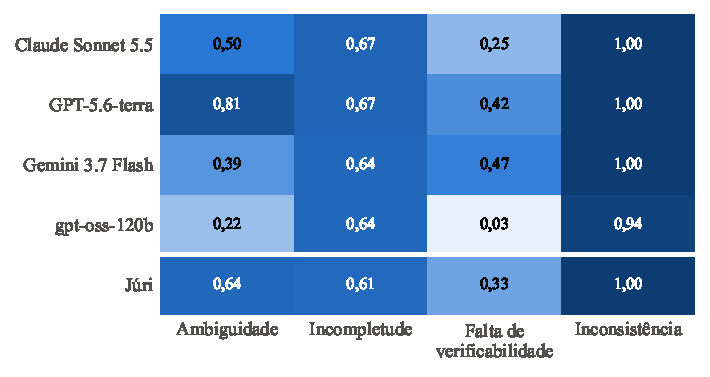
\includegraphics[width=0.75\textwidth]{fig1_deteccao.pdf}
\caption{Detecção exata do defeito injetado, por modelo e tipo de defeito}
\label{fig:deteccao}
\end{figure}

A falta de verificabilidade teve o maior descompasso: os modelos quase sempre pediram revisão, mas, somando os quatro, 48\% das respostas rotularam o defeito como ambiguidade e só 31\% como falta de verificabilidade (Figura~\ref{fig:confusao}). Termos como ``rapidamente'' e ``amigável'' são lidos como ambíguos, o que aponta uma fronteira pouco nítida entre os dois rótulos. Por outro lado, 33\% das respostas às variantes ambíguas não apontaram defeito algum.

\begin{figure}[ht]
\centering
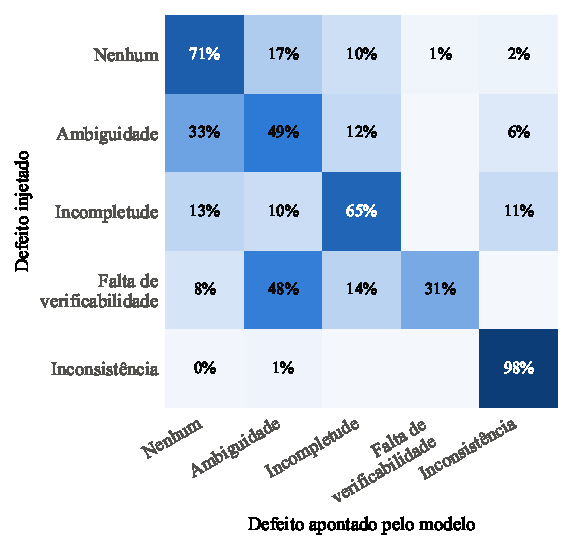
\includegraphics[width=0.62\textwidth]{fig5_confusao.pdf}
\caption{Defeito injetado (linhas) $\times$ defeito apontado (colunas), em \% das respostas de cada linha, somando os quatro modelos}
\label{fig:confusao}
\end{figure}

O rigor variou muito entre modelos (Figura~\ref{fig:fpfn}). Gemini (especificidade 1,00), gpt-oss-120b (0,94) e Claude (0,92) aceitaram quase todos os originais. O GPT-5.6-terra pediu revisão de 92\% deles (especificidade 0,08 \IC{0,00}{0,17}), apontando lacunas menores, como o ponto de início da contagem de um limite de 2 segundos, em geral rotuladas como ambiguidade. Isso explica a sua maior detecção exata de ambiguidade (0,81). O gpt-oss-120b fica no extremo oposto, com a maior taxa de falsos negativos (0,29). O macro-F1 foi maior no Gemini (0,68) e no júri (0,68), seguidos de Claude (0,64), GPT-5.6-terra (0,56) e gpt-oss-120b (0,49).

\begin{figure}[ht]
\centering
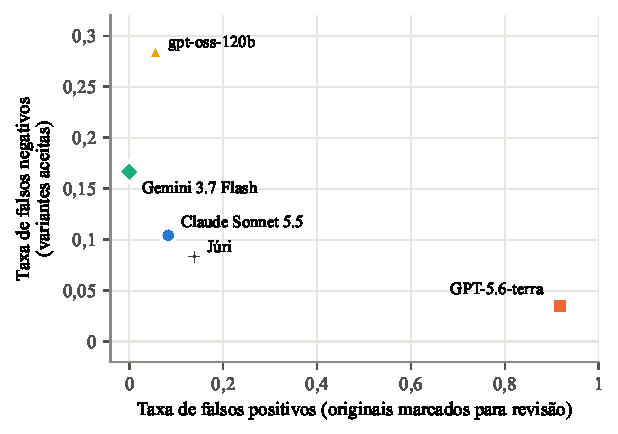
\includegraphics[width=0.62\textwidth]{fig2_fp_fn.pdf}
\caption{Taxa de falsos positivos (originais marcados para revisão) $\times$ taxa de falsos negativos (variantes aceitas)}
\label{fig:fpfn}
\end{figure}

Todos os modelos reduziram a nota no critério afetado (Figura~\ref{fig:queda}). No erro em relação à faixa esperada, o Claude teve o menor valor (MAE 0,21 \IC{0,13}{0,30}), seguido do júri (0,25); o gpt-oss-120b teve o maior (0,48), concentrado em ausência de ambiguidade.

\subsection{RQ2: robustez a mudanças superficiais}

O Claude foi o mais estável entre repetições: mesma decisão em 100\% dos itens, mesmo defeito em 98\% e alfa de 0,98. Seguiram-se Gemini (decisão 97\%; alfa 0,97), GPT-5.6-terra (93\%; 0,90) e gpt-oss-120b (88\%; 0,83), este com o mesmo defeito em só 75\% dos itens, apesar da temperatura 0.

As perturbações mudaram a nota em menos de 0,5 ponto em média (Figura~\ref{fig:robustez}). Para GPT-5.6-terra, Gemini e gpt-oss-120b, o efeito fica dentro do ruído entre repetições. A exceção é o Claude: com ruído de 0,05, a formatação elevou a variação para 0,13 e a mudança de ordem para 0,20, trocando a decisão em 8\% \IC{2\%}{17\%} dos itens e o defeito apontado em 12\%, contra 2\% entre repetições. O efeito das perturbações só se torna visível no modelo cujo ruído próprio é baixo.

\begin{figure}[ht]
\centering
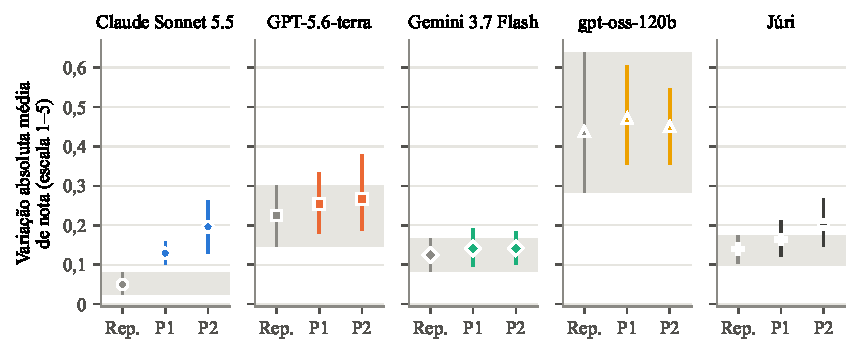
\includegraphics[width=\textwidth]{fig4_robustez.pdf}
\caption{Variação absoluta média de nota entre repetições (Rep.), com formatação alterada (P1) e com ordem alterada (P2), com IC 95\%. A faixa cinza é o IC do ruído entre repetições}
\label{fig:robustez}
\end{figure}

\subsection{RQ3: júri $\times$ modelos individuais}

O júri não superou o melhor modelo, mas ficou perto dele em todas as métricas. Empatou com o Gemini no maior macro-F1 (0,68), teve o segundo menor MAE (0,25) e uma taxa de falsos negativos (0,08) que é metade da do Gemini (0,17). Também neutralizou o modelo menos estável: sua variação de nota entre repetições (0,14) é um terço da do gpt-oss-120b (0,44). Em contrapartida, a especificidade do júri (0,86) ficou abaixo da de três modelos individuais, porque, com quatro juízes, dois votos bastam para ``revisar'' e o GPT-5.6-terra vota assim quase sempre.

A concordância entre modelos foi de 0,74 (alfa de Krippendorff), alta em consistência (0,89) e baixa em ausência de ambiguidade (0,57). O custo total foi de cerca de US\$~2,00 pelos preços de tabela (Claude $\approx$ US\$~0,97; GPT-5.6-terra $\approx$ 0,74; Gemini $\approx$ 0,26; gpt-oss-120b $\approx$ 0,05), com latência média entre 1,5\,s e 3,2\,s por chamada. O júri não exige chamadas extras; seu custo é a soma dos modelos.

\subsection{RQ4: dimensões mais difíceis}

A queda média de nota no critério afetado ordena as dimensões da mais difícil para a mais fácil: ambiguidade (1,04), incompletude (1,85), falta de verificabilidade (2,61) e inconsistência (3,72) (Figura~\ref{fig:queda}). A inconsistência com regras explícitas foi detectada e rotulada em quase todos os casos, com a maior concordância entre modelos. A ambiguidade teve a menor queda, a menor concordância e a menor proporção de variantes marcadas para revisão. A falta de verificabilidade combina queda grande com detecção exata baixa: o problema é percebido, mas recebe outro nome.

\begin{figure}[ht]
\centering
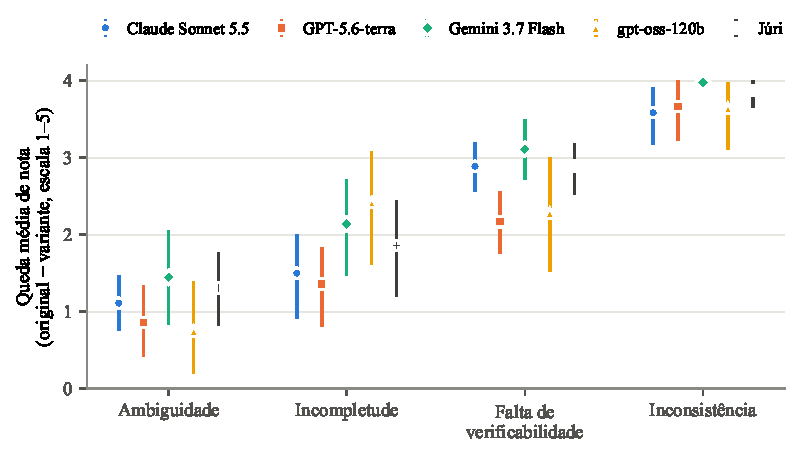
\includegraphics[width=\textwidth]{fig3_queda_nota.pdf}
\caption{Queda média de nota no critério afetado (original $-$ variante), com IC 95\%}
\label{fig:queda}
\end{figure}

\section{Discussão}

\textbf{Triagem sim, diagnóstico com cautela.} Os modelos são bons em separar requisitos com problema de requisitos corretos, desde que se escolha um modelo calibrado. São menos confiáveis para dizer qual é o problema, exceto quando ele contradiz uma regra explícita. Isso sugere usar LLMs como filtro de primeira passagem, com o diagnóstico final feito por um analista.

\textbf{Concordância não é acerto.} O padrão relatado por \citet{jain2025}, de juízes que aceitam bem e rejeitam mal, não se repetiu de forma uniforme: aqui, um modelo rejeitou quase tudo e outro aceitou demais. O rigor de cada modelo precisa ser medido com pares correto/defeituoso, e não inferido da concordância com outros juízes.

\textbf{O júri herda o viés do mais severo.} Diferentemente do ganho relatado por \citet{verga2024}, o júri ficou perto do melhor modelo sem superá-lo, em linha com \citet{williams2025}. A regra de agregação importa: com um juiz muito severo, a regra ``pelo menos metade'' desloca o júri para falsos positivos. Excluir o juiz descalibrado ou exigir maioria estrita são alternativas a testar.

\textbf{A taxonomia pesa.} A troca frequente entre ``ambiguidade'' e ``falta de verificabilidade'' sugere que parte da dificuldade está nos rótulos, e não na percepção. Um rubric com exemplos de fronteira entre essas categorias pode melhorar a detecção exata.

\textbf{LLMs como revisores do próprio benchmark.} Na execução-piloto, os modelos apontaram contradições reais em três requisitos que a equipe considerava corretos. O episódio ilustra o uso mais promissor observado: um segundo par de olhos que encontra o que passou despercebido, e não um árbitro final.

\section{Ameaças à validade}

\textbf{Validade interna.} O corpus foi construído pelos pesquisadores, com apoio de um LLM da mesma família de um dos juízes (Claude), o que pode favorecê-lo. Três bases foram corrigidas após a execução-piloto; a correção se limitou a contradições e omissões objetivas em relação às regras do contexto. As variantes incompletas são mais curtas por construção.
\textbf{Validade de construto.} O gabarito é operacional e assume que cada variante tem só o defeito injetado; a sobreposição entre ambiguidade e falta de verificabilidade mostra que essa separação nem sempre é nítida.
\textbf{Validade de conclusão.} Com 12 requisitos-base, os intervalos de confiança são largos, e diferenças pequenas entre modelos não são conclusivas.
\textbf{Validade externa.} Um único domínio, idioma (inglês) e redação de prompt foram usados, e todos os modelos foram acessados por um único intermediário. Modelos proprietários mudam com o tempo; os resultados valem para as versões e datas registradas.

\section{Conclusão}

Este trabalho apresentou um benchmark controlado para avaliar LLMs como juízes da qualidade de requisitos. Os quatro modelos avaliados perceberam a maioria dos defeitos, mas nomearam o defeito corretamente com frequência bem menor, exceto em inconsistências explícitas. A ambiguidade foi a dimensão mais difícil. O rigor variou do excesso de exigência ao excesso de aceitação, e mudanças superficiais no prompt tiveram efeito pequeno. O júri ficou perto do melhor modelo em todas as métricas, sem superá-lo.

Como trabalhos futuros, propõem-se: ampliar o corpus para outros domínios e idiomas; testar variações de prompt e rubrics com exemplos de fronteira entre categorias; avaliar regras de agregação e júris dinâmicos \citep{li2025jury}; incluir decision models \citep{li2026jev}; e comparar o rigor dos modelos com o de analistas humanos.

\textbf{Disponibilidade.} Corpus, prompts, configuração, scripts, respostas brutas e notebook de gráficos estão na pasta \texttt{benchmark/} do repositório do projeto.

\bibliographystyle{plainnat}
\bibliography{referencias}

\end{document}
